

\definecolor{codegreen}{rgb}{0,0.6,0}
\definecolor{codegray}{rgb}{0.5,0.5,0.5}
\definecolor{codepurple}{rgb}{0.58,0,0.82}
\definecolor{backcolour}{rgb}{0.95,0.95,0.92}

\lstdefinestyle{mystyle}{
    backgroundcolor=\color{backcolour},   
    commentstyle=\color{codegreen},
    keywordstyle=\color{magenta},
    numberstyle=\tiny\color{codegray},
    stringstyle=\color{codepurple},
    basicstyle=\ttfamily\footnotesize,
    breakatwhitespace=false,         
    breaklines=true,                 
    captionpos=b,                    
    keepspaces=true,                 
    numbers=left,                    
    numbersep=5pt,                  
    showspaces=false,                
    showstringspaces=false,
    showtabs=false,                  
    tabsize=2
}

\lstset{style=mystyle}

\chapter{Analisi della Realtà} % Main chapter title
\section*{1.1 \hspace{1cm} Analisi del Problema}
Molti Paesi hanno un modo diverso per distribuire l'energia elettrica. In Italia, per esempio, la Centrale Elettrica produce energia elettrica, che è distribuita ad una Cabina Elettrica ad alta tensione attraverso le Linee Elettriche che passano per i Tralicci.
Gli Stati Uniti, però, hanno un approccio diverso:
\begin{itemize}
    \item[1.] L'elettricità è prodotta in una centrale composta da generatori i quali possono utilizzare il vento, il carbone, il gas naturale o l'acqua.
    \item[2.] La corrente viene inviata ai trasformatori i quali alzano la tensione permettendo il trasferimento su lunghe distanze.
    \item[3.] L'elettricitá passa attraverso le linee di trasmissione ad alta tensione che si estendono in tutto il paese.
    \item[4.] Il flusso di corrente raggiunge una sottostazione, dove la tensione viene abbassata in modo da poter essere distribuita su linee elettriche più piccole.
    \item[5.] Queste linee si estendono nel centro cittadino dove trasformatori più piccoli riducono nuovamente la tensione per renderla utilizzabile nelle abitazioni. Questi trasformatori più piccoli possono essere montati sui tralicci o posizionati a terra.
    \item[6.] Si collega alle case e passa attraverso un contatore che misura il consumo di ogni cliente.
    \item[7.] L'elettricità arriva al pannello di servizio il quale é fornito dell'interruttore magneto-termico che apre la rete in caso di cortocircuito, chiusura del circuito a terra o sovraccarico.
    \item[8.] L'elettricità viaggia attraverso i fili all'interno dei muri fino alle prese e passa in tutta la casa.
\end{itemize}

Date queste differenze, solo le entità comuni a tutti i Paesi verranno memorizzate:
\begin{itemize}
    \item Centrale Elettrica
    \item Traliccio
    \item Cabina Elettrica (ad alta tensione)
    \item Linea Elettrica
\end{itemize}

Il Software Permetterà agli amministratori di sistema di effettuare operazioni CRUD (Create, Read, Update e Delete) sulle entità.

\section*{1.2 \hspace{1cm} L'azienda}
L'unica cosa che sappiamo della società è che è una società di distribuzione di Energia Elettrica. Dato che la traccia la descrive come "La Società" e non ci sta una specificazione riguardanti la nazione, considero che l'azienda ha un monopolio sul mercato dell'energia elettrica nel mondo intero, semplicemente per lavorare sul worst-case ovvero la "peggior situazione" possibile. \\

Dato che non viene specificata come deve essere memorizzata la posizione delle entità, userò il sistema di coordinate GPS. \\

Siccome non viene specificato chi può accedere l'archivio, considero che solo gli amministratori di sistema possono accederci. Gli amministratori possono inserire ed eliminare i dati direttamente dalla pagina web dell'archivio, accessibile solo a loro. \\

Per fare l'autenticazione alla piattaforma, gli impiegati devono inserire le loro credenziali, e poi fare il riconoscimento facciale per confermare la loro identita'.

L'archivio sarà popolato originariamente con dati ufficiali da NASA, data.europa.eu, etc., e verranno citati nel codice sorgente. \\




\section*{1.3 \hspace{1cm} L'infrastruttura}
L'azienda ha varie sedi sparse nel mondo, i server sono collocati nel mare (\href{https://datacenterfrontier.com/microsoft-servers-in-our-underwater-data-center-are-super-reliable/#:~:text=Microsoft%3A%20Servers%20in%20Our%20Underwater%20Data%20Center%20Are%20Super%2DReliable,-By%20Rich%20Miller&text=Microsoft%20recently%20retrieved%20the%20Project,the%20Orkney%20Islands%20in%20Scotland}{come fa microsoft}) aumentando cosí l'efficenza e riducendo i costi, essi sono anche divisi in diversi sotto domini tutti connessi allo stesso database. \\
Il DBMS scelto é PostgreSQL, per la sua scalabilitá esponenziale e per il supporto alla distribuzione in piú cluster. \\

Nell'analisi del problema sono presenti diversi sottodomini,  quelli sviluppati in questo progetto sono:
\begin{itemize}
    \item https://www.electrocorp.com/
    \item https://admin.electrocorp.com/
    \item https://api.electrocorp.com/
    \item https://mail.electrocorp.com/
\end{itemize}
(www.electrocorp.com risulta giá registrato da un'azienda non affiliata con questo progetto. Per questo il dominio deve essere sovrascritto in /etc/hosts per modificare il reindirizzamento al progetto, non puó essere applicato ad una macchina esterna alla rete). \\ \\
I server utilizzano come OS SUSE Linux, una distribuzione Enterprise di GNU/Linux pensata per i server.

La rete si compone di diverse sottoreti, una per ogni cluster, tutte gestite da Kubernetes. \\
Ogni sottorete é protetta da alcune regole firewall, di seguito la lista:
\begin{center}
    \begin{tabular}{ |l|c|c|c|c|c| } 
        \hline
        \multicolumn{6}{|c|}{Firewall on www.electrocorp.com} \\
        \hline
            Number & Protocol & Source IP     & Destination IP & Destination Port & Action \\
        \hline
            4      & ALL      & 0.0.0.0/0    & 0.0.0.0/0     & 0-65535          & ACCEPT \\
        \hline
    \end{tabular}
\end{center}
    
\begin{center}
    \begin{tabular}{ |l|c|c|c|c|c| } 
        \hline
        \multicolumn{6}{|c|}{Firewall on admin.electrocorp.com} \\
        \hline
            Number & Protocol & Source IP     & Destination IP & Destination Port & Action \\
        \hline
            1      & TCP      & 172.22.3.0/24 & 172.22.4.0/24  & 5432             & ACCEPT \\
            2      & TCP      & 32.1.0.0/16   & 172.22.3.0/24  & 443              & ACCEPT \\
            3      & ALL      & 0.0.0.0/0    & 0.0.0.0/0     & 0-65535          & DROP \\
        \hline
    \end{tabular}
\end{center}

\begin{center}
    \begin{tabular}{ |l|c|c|c|c|c| } 
        \hline
        \multicolumn{6}{|c|}{Firewall on api.electrocorp.com} \\
        \hline
            Number & Protocol & Source IP     & Destination IP & Destination Port & Action \\
        \hline
            4      & ALL      & 0.0.0.0/0    & 172.22.2.5     & 0-65535          & ACCEPT \\
        \hline
    \end{tabular}
\end{center}

La sottorete 32.1.0.0/16 é gestita dalla compagnia ed é usata per permettere agli impiegati di connettersi all'area ristretta attraverso un RDP.

\begin{center}
    \begin{tabular}{ |l|c|c|c|c|c| } 
        \hline
        \multicolumn{6}{|c|}{Firewall on the DBMS cluster} \\
        \hline
            Number & Protocol & Source IP     & Destination IP & Destination Port & Action \\
        \hline
            1      & TCP      & 172.22.2.0/24 & 172.22.4.0/24  & 5432             & ACCEPT \\
            2      & TCP      & 172.22.4.0/24 & 172.22.4.0/24  & 5432             & ACCEPT \\
            3      & ALL      & 0.0.0.0/0    & 0.0.0.0/0     & 0-65535          & DROP  \\
        \hline
    \end{tabular}
\end{center}

Di seguito la configurazione dei router (firewall, port forwarding) che girano Linux.

\lstinputlisting{Code/networking.sh}

Gli host nella stessa sottorete possono solo interagire fra loro e con il DBMS cluster. \\

Questo é il docker-compose.yml, file di configurazione, che identifica anche le varie sottoreti.

\lstinputlisting{../../../project/docker-compose.yml}

... e il file /etc/hosts (C: \textbackslash Windows \textbackslash system32 \textbackslash etc \textbackslash hosts)
\lstinputlisting{/etc/hosts}

\newpage
Ed ecco lo schema di rete:
\begin{figure}[H]
    \centering
    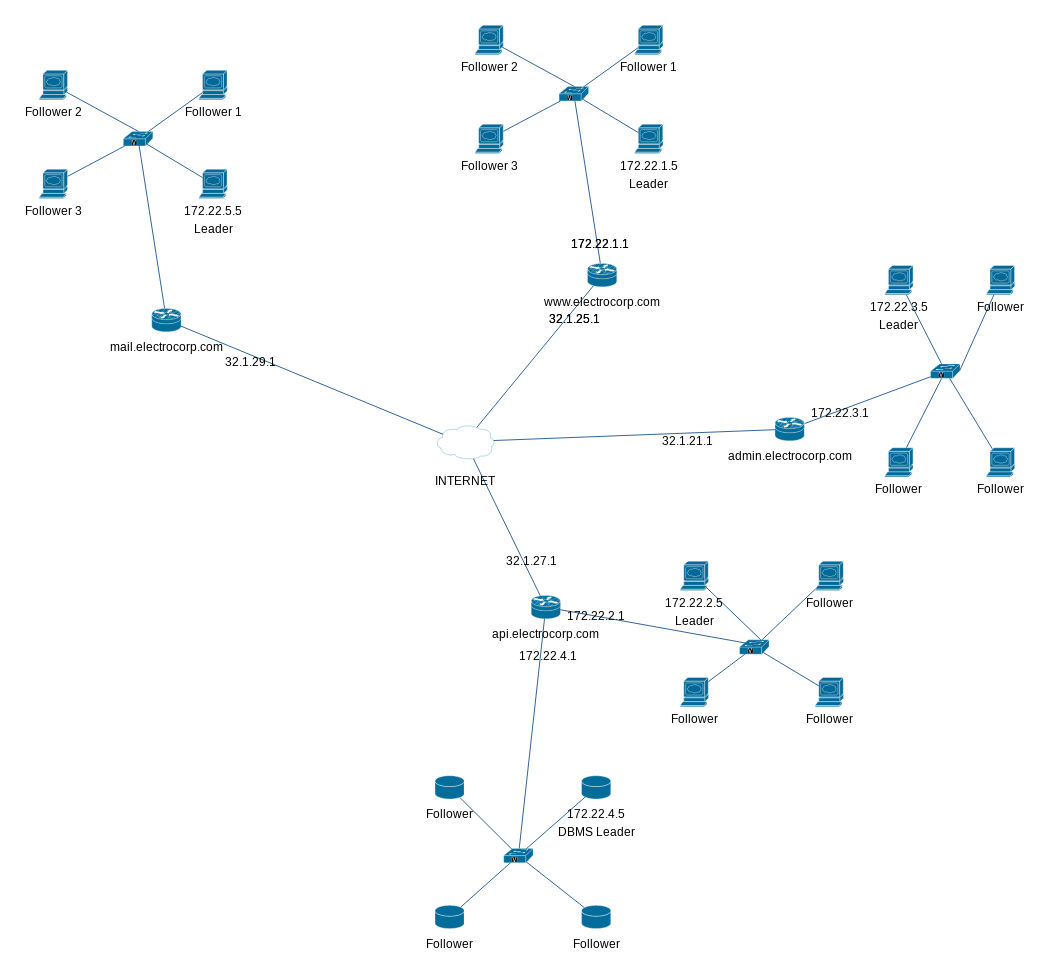
\includegraphics[width=\linewidth]{Figures/Rete.png}
\end{figure}
    
\section*{1.4 \hspace{1cm} Il sito}
Il database é accessibile solo agli amministratori di sistema, i quali possono navigare, aggiungere, eliminare e modificare i dati dallo stesso. \\

Gli amministratori di sistema possono anche gestire i ruoli e gli utenti. \\


Queste sono le regole di accesso per gli utenti su ogni sito.
\begin{center}
    \begin{tabular}{ |l|c|c|c|c|c| } 
        \hline
        \multicolumn{6}{|c|}{Access Control (admin.electrocorp.com)} \\
        \hline
                                        & Archive    & Control Panel            & Login        & Finances                & Logs \\
        \hline
            \textbf{Administrator}      & ALL        & ALL                      & AUTHENTICATE & ALL                     & READ \\
            \textbf{Finances}           &            &                          & AUTHENTICATE & ALL                     &  \\
            \textbf{*not auth*}         &            &                          & AUTHENTICATE &                         &  \\
        \hline
    \end{tabular}
\end{center}
Accessibile solo dagli impiegati. \\


Questo e' il diagramma a blocchi. \\
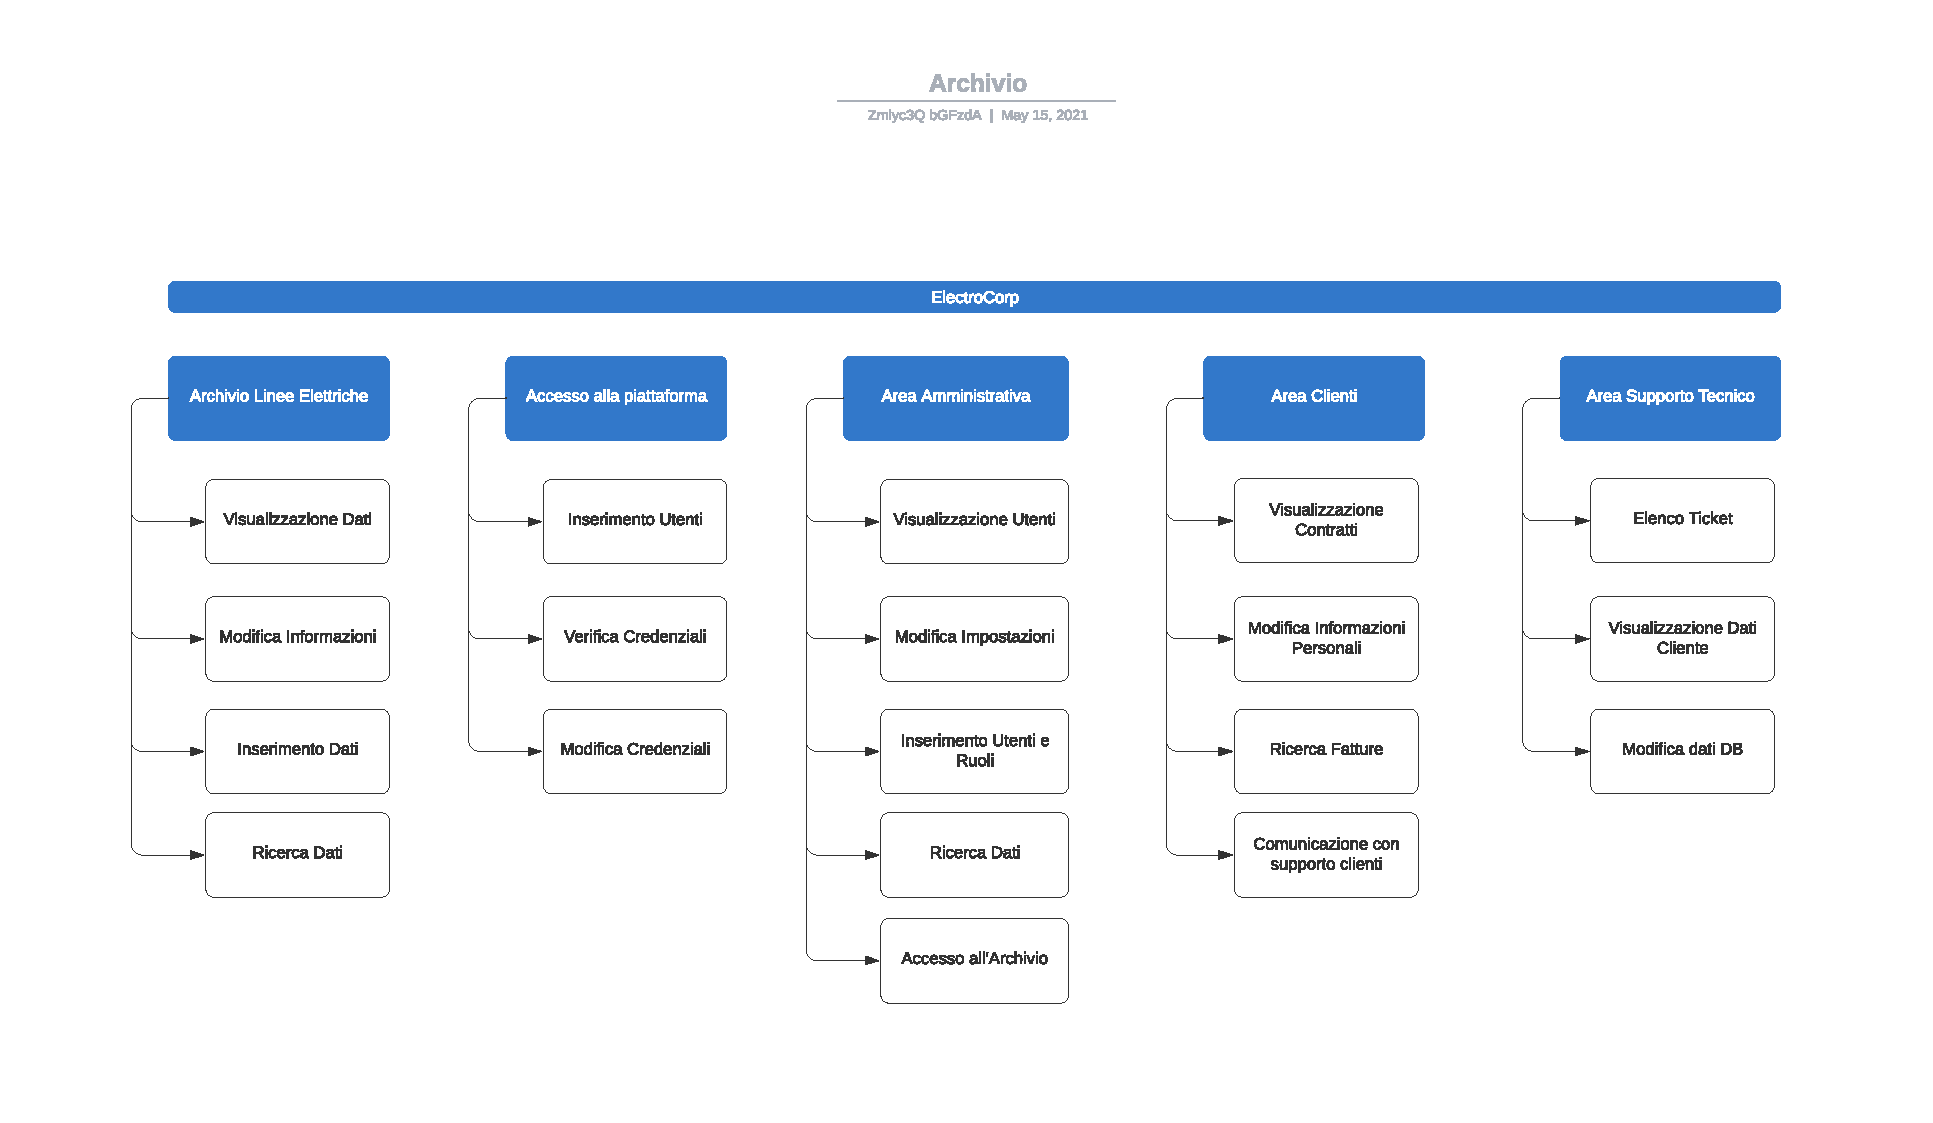
\includepdf{Figures/blocks.pdf}

E questo e' il flow chart.
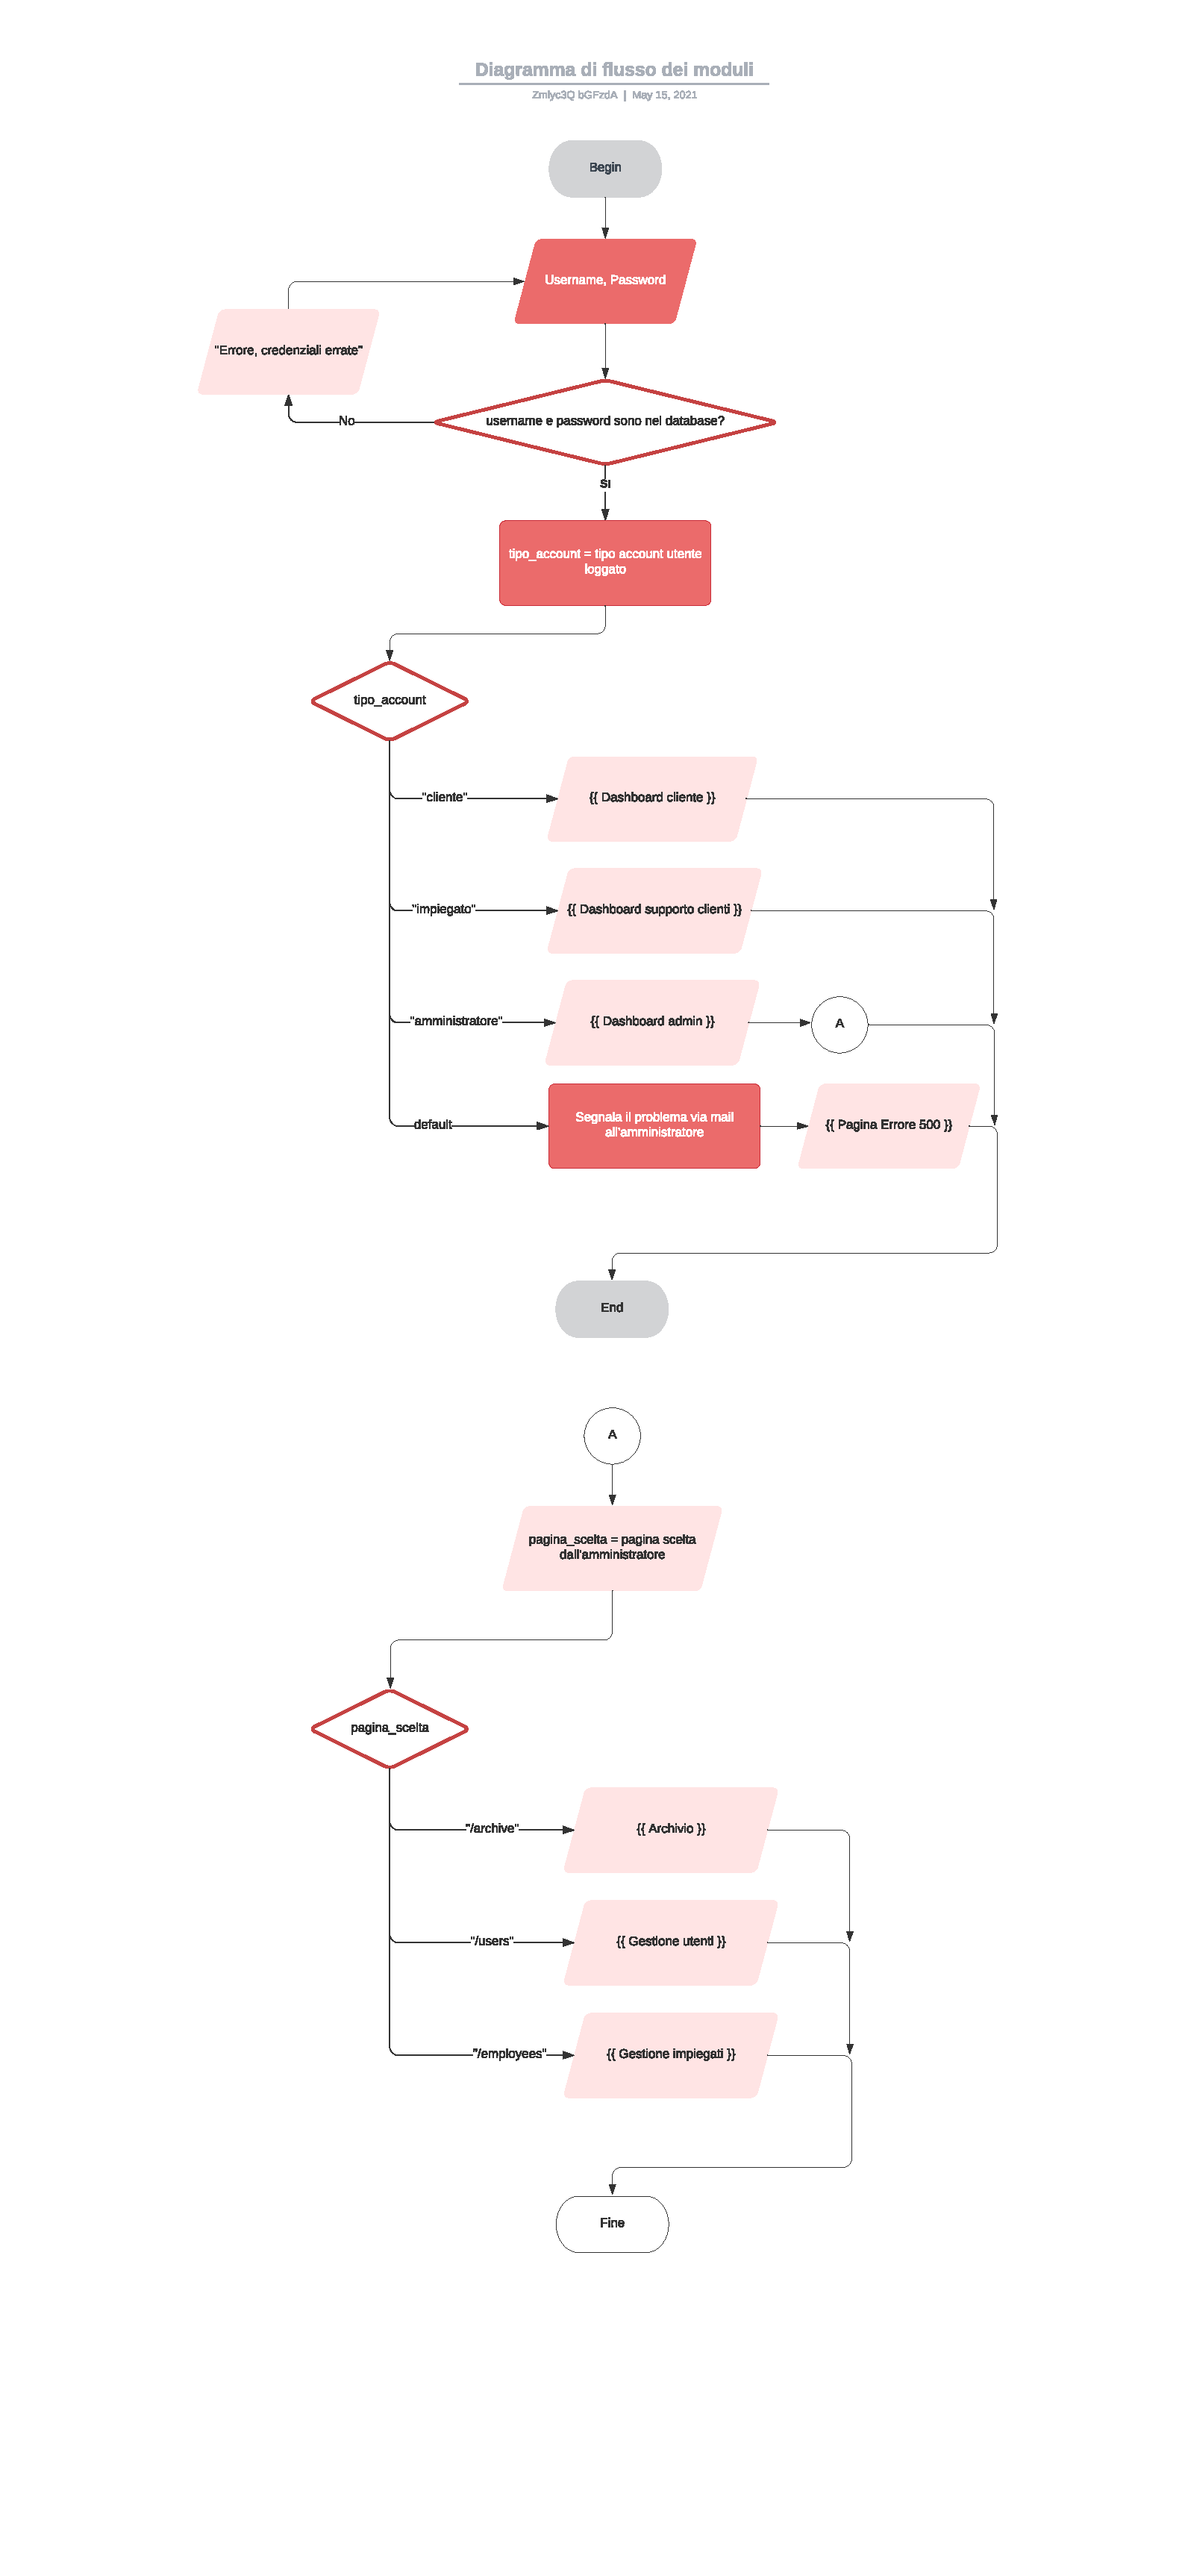
\includepdf{Figures/flow_chart.pdf}